% !BIB program = bibtex
% !TeX spellcheck = ru_RU

% About magic macros see also
% https://tex.stackexchange.com/questions/78101/

% По умолчанию используется шрифт 14 размера.
% Если Вы не влезаете в лимит страниц и нужен 12-й шрифт,
% то уберите опцию [14pt]
\documentclass[14pt, russian]{matmex-diploma-custom}

%%% Обязательные пакеты
%% Beamer
\usepackage{beamerthemesplit}
\usetheme{SPbGU}
\beamertemplatenavigationsymbolsempty
\usepackage{appendixnumberbeamer}

%% Локализация
\usepackage{fontspec}
\setmainfont{CMU Serif}
\setsansfont{CMU Sans Serif}
\setmonofont{CMU Typewriter Text}
%\setmonofont{Fira Code}[Contextuals=Alternate,Scale=0.9]
%\setmonofont{Inconsolata}
% \newfontfamily\cyrillicfont{CMU Serif}

\usepackage{polyglossia}
\setdefaultlanguage{russian}
\setotherlanguage{english}
\usepackage[autostyle]{csquotes} % Правильные кавычки в зависимости от языка

%% Графика
\usepackage{wrapfig} % Позволяет вставлять графику, обтекаемую текстом
\usepackage{pdfpages} % Позволяет вставлять многостраничные pdf документы в текст

%% Математика
\usepackage{amsmath, amsfonts, amssymb, amsthm, mathtools} % "Адекватная" работа с математикой в LaTeX

% Математические окружения с русским названием
\newtheorem{rutheorem}{Теорема}
\newtheorem{ruproof}{Доказательство}
\newtheorem{rudefinition}{Определение}
\newtheorem{rulemma}{Лемма}

%%% Дополнительные пакеты. Используются в презентации, но могут быть отключены при необходимости
\usepackage{tikz} % Мощный пакет для создание рисунков, однако может очень сильно замедлять компиляцию
\usetikzlibrary{decorations.pathreplacing,calc,shapes,positioning,tikzmark}

\usepackage{multirow} % Ячейка занимающая несколько строк в таблице

%% Пакеты для оформления алгоритмов на псевдокоде
\usepackage[noend]{algpseudocode}
\usepackage{algorithm}
\usepackage{algorithmicx}

\usepackage{fancyvrb}

\NewDocumentCommand{\xxHash}{}{\textsc{xxHash}}
\NewDocumentCommand{\riscv}{}{\textsc{RISC-V}}
\NewDocumentCommand{\xxh}{m}{\textsc{XXH{#1}}}
\NewDocumentCommand{\sew}{}{\textsc{SEW}}
\NewDocumentCommand{\vl}{}{\textsc{VL}}
\NewDocumentCommand{\rvv}{}{\textsc{RVV}}
\usepackage{booktabs}
\usepackage{tabularx}
\usepackage{siunitx} % для таблиц с единицами измерений


% \usepackage{lineno}
% \linenumbers

\usepackage{xurl}

\begin{document}
\input{title.tex}
\maketitle
\setcounter{tocdepth}{2}
\tableofcontents

% !TeX spellcheck = ru_RU
% !TEX root = vkr.tex

\section*{Введение}
\thispagestyle{withCompileDate}

Сложно представить курс по информатике без практических заданий: они позволяют лучше усвоить и закрепить теоретический материал.
К сожалению, на проверку заданий у преподавателя может уходить довольно много времени, а контрольные цифры приема на специальности, связанные с информационными технологиями, увеличиваются каждый год~\cite{2024GoduKolichestvo}.
Некоторые преподаватели решают данную проблему, привлекая других проверяющих, например старшекурсников, но данный подход не является идеальным: по наблюдениям кафедры системного программирования на каждые 4--5 человек нужен один проверяющий.
Поиск такого количества людей является непростой задачей.

Курс по теории формальных языков является важной частью обучения IT-специалиста.
Формальные языки находит своё применение как в теоретических областях, таких как математическая логика~\cite{guhaParikhAutomataInfinite2022,draghiciSemEnovArithmetic2023a}, так и в прикладных: при написании парсеров~\cite{gruneParsingTechniques2008, scottGLLParsing2010}, в графовых базах данных~\cite{hellingsQueryingPathsGraphs2016,noleRegularPathQueries2016}, в биоинформатике~\cite{dyrkaEstimatingProbabilisticContextfree2019,wjandersonEvolvingStochasticContext2012}.

На математико-механическом факультете СПбГУ так же читается данный курс.
В нём имеется 12 практических заданий.
В большинстве задач требуется реализовать нетривиальный алгоритм: это вызывает сложности как у студентов, так как требуется аккуратность при выполнении, так и у проверяющих, ведь для проверки необходимо разобраться в коде студента.
Студенты обязаны предоставлять рукописные тесты к каждой задаче, но тестовое покрытие не всегда описывает все крайние случаи, поэтому иногда студентам удается сдать не корректное решение.

Тем не менее алгоритмические задачи довольно часто поддаются property-based тестированию, так как известны свойства входных и выходных данных.
Таким образом было принято решение автоматизировать проверку задач, используя property-based тесты.

% !TeX spellcheck = ru_RU
% !TEX root = vkr.tex

\section{Обзор}
\label{sec:relatedworks}
\subsection[Векторное расширение RISC-V]{Векторное расширение \riscv{}}
Векторное расширение \riscv{} находилось в разработке довольно долго, из-за чего производители чипов начали выпускать свои решения основываясь на недоработанной версии стандарта 0.7.1.
Один из таких чипов~--- \textsc{Allwinner D1}, получил большое распространение в недорогих одноплатных ПК, таких как \textsc{Sipeed Lichee RV} и \textsc{MangoPi MQ-Pro}.

Последней и официальной ратифицированной версией является версия 1.0.

% !TeX spellcheck = ru_RU
% !TEX root = vkr.tex

\section{Постановка задачи}
\label{sec:task}

Целью работы является разработка инфраструктуры для автоматизации проверки задач по курсу \enquote{Теория формальных языков}.
Для её выполнения были поставлены следующие задачи:
\begin{enumerate}
    \item Изучить способы автоматического тестирования учебных задач~(раздел~\ref{subsec:types}).
    \item Создать базовую инфраструктуру для автоматического тестирования~(раздел~\ref{subsec:infra}).
    \item Произвести проверку автоматических тестов, путём реализации решений~(раздел~\ref{subsec:slns}).
    \item Исправить накопленный технический долг~(раздел~\ref{subsec:housekeeping}). \note{by Kakadu, выглядит слегка кринжово, но я тоже ничего лучше придумать не могу}
          \begin{enumerate}
              \item Сменить систему управления зависимостями.
              \item Обновить зависимости.
          \end{enumerate}
\end{enumerate}

% !TeX spellcheck = ru_RU
% !TEX root = vkr.tex

% !TeX spellcheck = ru_RU
% !TEX root = vkr.tex

\section{Общая архитектура проекта}
\label{sec:big-arch}

Проект \Lamagraph{} ставит перед собой цель изучить возможности по созданию специализированных ускорителей на основе \INs{}.

К проекту выдвинуты следующие требования.
\begin{itemize}
    \item Возможность параметризовать компилятор и вычислительное ядро типами агентов сети и правилами их редукции.
    \item Возможность сбора статистики такой, как размер сети, количество редукций, время исполнения и другой.
    \item Возможность постановки сравнительных экспериментов.
    \item Использование единого стека технологий~--- гомогенность.
    \item Получение полнофункционального прототипа, содержащего все компоненты, важнее, чем детальная проработка какого-то отдельного компонента.
    \item Расширяемость и модифицируемость.
          Должна быть возможность вносить изменения в любые компоненты.
\end{itemize}


Крупномасштабная архитектура проекта изображена на рисунке~\ref{fig:lamagraph-big} и состоит из трёх крупных блоков.
\begin{description}
    \item[Compiler] Транслятор ML-подобного языка программирования.
          Содержит в себе интерпретатор и генерирует промежуточное представление, пригодное к дальнейшей трансляции в \INs{}.
    \item[Hardware] Генератор описания аппаратуры для ПЛИС, параметризуемый базисом агентов сети.
    \item[Middle] Транслятор из промежуточного представления в байт-код, пригодный для исполнения на процессоре, сгенерированном в блоке Hardware.
\end{description}


Проект является командным.
Блоки Compiler и Hardware достаточно независимы друг от друга.
Блок Middle объединяет два других, поэтому его разработка должна быть скоординирована.
В данной работе речь пойдёт о блоке Compiler.

\begin{figure}
    \begin{center}
        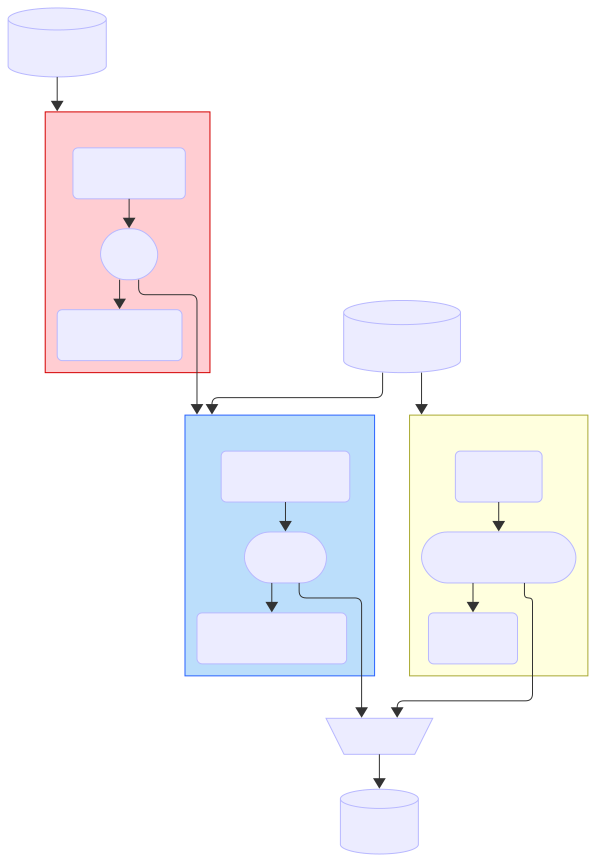
\includegraphics[width=0.6\linewidth]{lamagraph-big}
    \end{center}
    \caption{Общая архитектура проекта \Lamagraph{}.}
    \label{fig:lamagraph-big}
\end{figure}

% !TeX spellcheck = ru_RU
% !TEX root = vkr.tex

\section{Подробности реализации}

В качестве языка реализации проекта был выбран \Haskell{}.
Предполагаемая архитектура изображена на рисунке~\ref{fig:lmlcmods}.

Для сборки проекта и версионирования зависимостей используется \textsc{Stack}\footnote{Сайт проекта: \url{https://docs.haskellstack.org/en/stable/} (дата обращения \DTMdate{2025-02-25})}, каждая часть, описанная в разделе~\ref{sec:big-arch}, является отдельным пакетом.
Для тестирования используется фреймворк \textsc{Tasty}\footnote{Описание проекта на \textsc{Hackage}: \url{https://hackage.haskell.org/package/tasty/} (дата обращения \DTMdate{2025-02-25})}, по умолчанию все части компилятора покрываются golden\footnote{Описание golden тестов: \url{https://ro-che.info/articles/2017-12-04-golden-tests} (дата обращения \DTMdate{2025-02-25})} тестами.

\begin{figure}[h]
    \begin{center}
        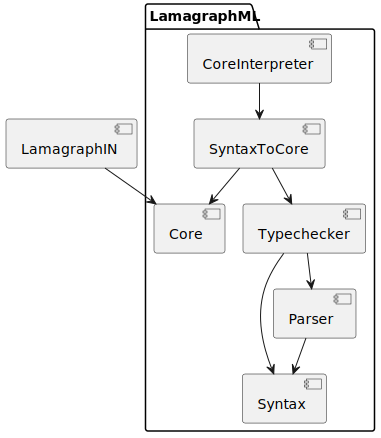
\includegraphics{components}
    \end{center}
    \caption{Архитектура транслятора}
    \label{fig:lmlcmods}
\end{figure}

\paragraph{Синтаксис языка.}

Синтаксис языка основан на \OCaml{}.
Однако упрощен для простоты реализации\footnote{С полной грамматикой можно ознакомиться в репозитории проекта: \url{https://github.com/Lamagraph/interaction-nets-in-fpga/blob/main/lamagraph-compiler/src/Lamagraph/Compiler/Syntax.hs} (дата обращения \DTMdate{2025-02-25})}.
Так, например в языке остались стандартные для функциональных языков конструкции, такие как сопоставление с образцом, рекурсивные и взаимнорекурсивные функции, а также алгебраические типы данных.
Однако в отличие от \OCaml{} отсутствует поддержка классов и функторов, а система модулей максимально упрощена и напоминает систему модулей в F\#.

Для представления AST (дерева абстрактного синтаксиса) используется паттерн Trees That Grow (TTG)~\cite{shayannajdTreesThatGrow}.
Он позволяет с помощью механизма type families~\cite{schrijversTypeCheckingOpen2008} гибко параметризовать дерево необходимыми аннотациями, более того аннотации могут различаться в разных узлах дерева, тем самым поддерживая безопасность кода.

\paragraph{Парсер.}

Для синтаксического анализа используется связка лексера \textsc{Alex} и парсер-генератора \textsc{Happy}, которые являются аналогами \textsc{flex} и \textsc{bison}, написанными на \Haskell{}.

На данном этапе аннотации с помощью TTG не используются.

Для тестирования лексера используются модульные тесты.
Для парсера используется property-based тестирование с использованием библиотеки \textsc{Hedgehog}\footnote{Репозиторий проекта: \url{https://github.com/hedgehogqa/haskell-hedgehog/} (дата обращения: \DTMdate{2025-02-19})}.
Данный метод основан на том, что синтаксический анализ в AST и печать AST должны давать тождественное отображение при композиции.

\paragraph{Вывод типов.}

Поскольку язык ML-подобный, используется система типов Хиндли-Милнера~\cite{hindleyPrincipalTypeSchemeObject1969, milnerTheoryTypePolymorphism1978}.

На данном этапе в аннотациях TTG сохраняется тип каждого узла дерева.

\paragraph{Промежуточное представление.}

AST получаемый после парсинга и вывода типов получается достаточно сложным~--- в нём большое количество различных узлов с аннотациями.
Для упрощения дальнейшей работы используется промежуточное представление на основе GHC Core\footnote{Подробнее можно прочитать по ссылке: \url{https://gitlab.haskell.org/ghc/ghc/-/wikis/commentary/compiler/core-syn-type} (дата обращения: \DTMdate{2025-02-19})}, также часто называемое обогащённым $\lambda$-исчислением\footnote{Подробнее узнать про способы обогащения $\lambda$-исчисления можно в~\cite[раздел~3.2]{peytonjones1987the}}.
Его описание представлено на листинге~\ref{lst:core}.

\begin{listing}
    \inputminted[fontsize=\footnotesize]{haskell}{figures/core.hs}
    \caption{Представление Core в алгебраических типах данных.}
    \label{lst:core}
\end{listing}

Важными отличиями от GHC Core являются наличие выделенного конструктора для пар, а также отсутствие типизации.

Наличие выделенного конструктора для пар обусловлено различием между ML и \Haskell{}~--- в первом пары тоже выделены и могут быть какой угодно арности, во втором же пара является синтаксическим сахаром для алгебраического типа-суммы и ограничена арностью 63.

От типизации пришлось отказаться в угоду простоты реализации, а также в виду отсутствия оптимизаций со стороны компилятора, где наличие типов упрощает и делает более безопасным их применение.

\paragraph{Трансляция высокоуровневого AST в промежуточное представление.}

Алгоритм трансляции достаточно прямолинеен, наиболее сложной частью является трансляция сложных шаблонов в левой части let-связывания и замена вложенных шаблонов на вложенные match-выражения.

% !TeX spellcheck = ru_RU
% !TEX root = vkr.tex

\section{Тестирование транслятора}

\begin{figure}[h]
    \begin{center}
        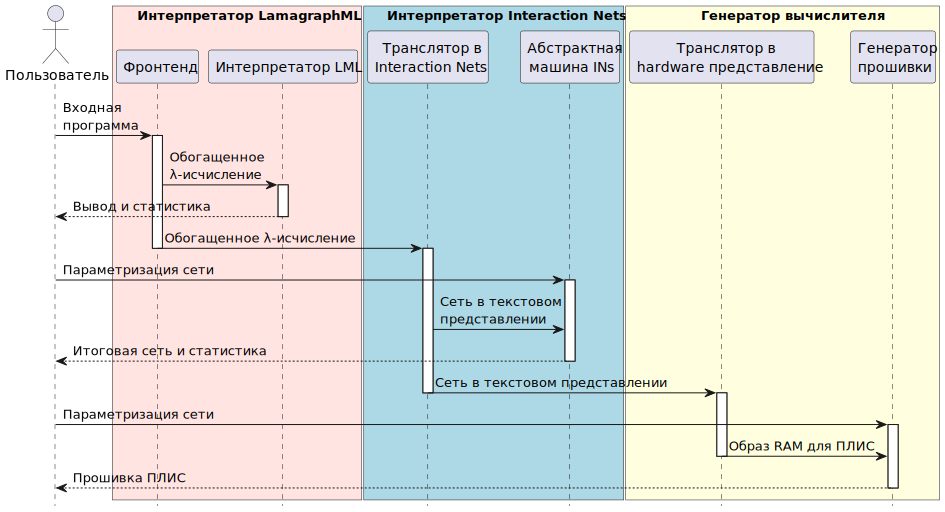
\includegraphics[width=0.9\linewidth]{using.pdf}
    \end{center}
    \caption{Диаграмма взаимодействия пользователя с программно-аппаратным стеком Lamagraph.}
    \label{fig:using}
\end{figure}

На данном этапе развития проекта проведение сравнительных экспериментов невозможно, тем не менее пользователь уже может взаимодействовать с инструментом.

Так, передав на вход программу на \LamagraphML{} пользователь может получить вывод интерпретатора, а также вывод абстрактной машины и соответствующую статистику, что проиллюстрировано на рисунке~\ref{fig:using}.

\subsection*{Анализ текущих возможностей}

Анализ проводился с учётом реализованной схемы трансляции чистого $\lambda$-исчисления в \INs{} со стратегией call-by-value.
Для вычисления использовались два набора правил: для последовательного вычисление аргументов применения и для параллельного.
Оба набора описаны в~\cite{sinotCallbyNameCallbyValueTokenPassing2005} и отличаются лишь правилом для взаимодействия агентов $\Downarrow$ и $a$.

\paragraph{Допустимые термы.}
Для проведения анализа было написано 10 программ.
Первоначально планировалось писать программы только на высокоуровневом \LamagraphML{}, однако в процессе выяснилось, что не все термы, используемые в бестиповом $\lambda$-исчислении могут быть протипизированы в системе типов Хиндли-Милнера без использования алгебраических типов данных (например, терм \texttt{pred}\footnote{Подробности можно прочитать в заметке Олега Киселева: \url{https://okmij.org/ftp/Computation/lambda-calc.html\#predecessor} (дата обращения: \DTMdate{2025-05-22})}).
Поэтому часть программ была вручную написана на бестиповом Core.
Кроме того, для корректного завершения программ в стратегии call-by-value условные конструкции необходимо было сделать \enquote{отложенными}, введя дополнительную $\lambda$-абстракцию\footnote{Более подробная мотивация такого подхода описана по ссылке: \url{https://cs.stackexchange.com/a/121350} (дата обращения: \DTMdate{2025-05-22})}.

Данная проблема~--- одна из самых важных для проекта на данный момент, поскольку Core и \INs{} планировалось использовать, как промежуточные представления, предоставляя пользователю только \LamagraphML{} и соответствующие возможности высокоуровневого языка.

Один из вариантов решения данной проблемы~--- введение числовых литералов, примитивных арифметических операцией и сопоставления с образцом.
Такое решение потребует расширения набора агентов и правил редукции, с учётом того, что арифметические операции строгие (eager) в своих аргументах.
Кроме того, необходимо изучить, каким образом возможна реализации такого расширения в компоненте Hardware.

\paragraph{Корректность результата.}
\begin{listing}
    \inputminted[fontsize=\footnotesize, breaklines]{ocaml}{figures/iterFactZero.lml}
    \caption{\texttt{IterFact(0)}, реализованный на \LamagraphML{}}
    \label{lst:iterFactZero}
\end{listing}
При анализе получаемых сетей была выявлена ещё одна проблема: call-by-value стратегия по определению не редуцирует под $\lambda$-абстракцией из-за чего получаемые сети довольно сложно анализировать на корректность ответа.

Так, например, в нотации из~\cite{fernandezCalculusInteractionNets1999}, результат вычисления итеративного факториала от 0 (см. листинг~\ref{lst:iterFactZero}) выглядит, как
\[\big\langle \Uparrow(\lambda(f, \lambda(x, a(f, x)))) \mid \big\rangle,\]
а для факториала от 1 уже так:
\begin{multline*}
    \big\langle \Uparrow(\lambda(f, \lambda(x, a(a(\lambda(c(u, v), \lambda(w, a(u, a(a(\lambda(\varepsilon, \lambda(z, z)), v), w)))), \\
    a(\lambda(t, \lambda(r, a(t, r))), f)), x)))) \mid \big\rangle.
\end{multline*}

В качестве решения проблемы можно, как уже упоминалось выше, добавить поддержку числовых литералов.
Также можно попробовать транслировать сеть обратно в $\lambda$-терм и осуществить оставшиеся редукции руками или с помощью интерпретатора, реализующего порядок вычислений, редуцирующий внутри $\lambda$-абстракции.

Отдельного внимания заслуживает мысль о смене схемы трансляции и использовании другой стратегии редукции.
С учётом существования нескольких способов кодирования \enquote{оптимальной} редукции~\cite{lampingAlgorithmOptimalLambda1990, aspertiBolognaOptimalHigherorder1996, gonthierGeometryOptimalLambda1992, vincentvanoostromLambdascopeAnotherOptimal2004}, смена стратегии вычислений может позволить редуцировать сети до нормальный формы, соответствующего $\lambda$-терма.

\paragraph{Сбор статистики.}
Поскольку \INs{}~--- параллельная модель вычислений, то при сборе статистики абстрактной машины нам было интересно не только количество малых шагов, но и метрики, связанные с параллельностью: количество больших шагов и максимальная ширина большого шага.

Здесь под \enquote{малым шагом} подразумевается редукция одной активной пары, под \enquote{большим шагом}~--- редукция, при которой сокращаются все возможные активные пары.
Под \enquote{шириной большого шага} имеется в виду количество малых шагов в одном большом.
Больших шагов совершается много, и каждый имеет свою ширину, поэтому в статистику попадает только максимальная ширина большого шага.

Отдельно стоит отметить, что последовательная и параллельная схема вычисления аргументов~--- это объекты уровня \INs{}, а большой и малый шаги~--- уровня абстрактной машины.
Таким образом последовательная схема вычисления тоже имеет большие шаги шириной больше одного, но они вызваны не самой стратегией вычисления $\lambda$-термов, а вспомогательными агентами, например, дупликаторами.

\begin{table}
    \footnotesize
    \begin{center}
        \begin{tabular}{lcrrr}
            \toprule
            Терм                                                                      &
            \multicolumn{1}{p{2.5cm}}{\raggedright Параллельная стратегия}            &
            \multicolumn{1}{p{2.3cm}}{\raggedright Количество малых шагов}            &
            \multicolumn{1}{p{3.7cm}}{\raggedright Максимальная ширина большого шага} &
            \multicolumn{1}{p{2.7cm}}{\raggedright Количество больших шагов}                                  \\
            \midrule
            \texttt{RecFact(0)}                                                       & Нет & 472  & 18 & 103 \\
            \texttt{RecFact(0)}                                                       & Да  & 498  & 18 & 111 \\
            \midrule
            \texttt{RecFact(1)}                                                       & Нет & 274  & 13 & 85  \\
            \texttt{RecFact(1)}                                                       & Да  & 302  & 12 & 94  \\
            \midrule
            \texttt{RecFact(2)}                                                       & Нет & 291  & 13 & 91  \\
            \texttt{RecFact(2)}                                                       & Да  & 321  & 12 & 101 \\
            \midrule
            \texttt{IterFact(0)}                                                      & Нет & 179  & 12 & 61  \\
            \texttt{IterFact(0)}                                                      & Да  & 199  & 12 & 62  \\
            \midrule
            \texttt{IterFact(1)}                                                      & Нет & 265  & 9  & 176 \\
            \texttt{IterFact(1)}                                                      & Да  & 323  & 11 & 124 \\
            \midrule
            \texttt{IterFact(2)}                                                      & Нет & 607  & 12 & 295 \\
            \texttt{IterFact(2)}                                                      & Да  & 703  & 14 & 190 \\
            \midrule
            \texttt{IterFact(3)}                                                      & Нет & 1097 & 22 & 414 \\
            \texttt{IterFact(3)}                                                      & Да  & 1231 & 22 & 256 \\
            \midrule
            \texttt{IterFact(4)}                                                      & Нет & 1766 & 33 & 533 \\
            \texttt{IterFact(4)}                                                      & Да  & 1938 & 33 & 322 \\
            \midrule
            \texttt{IterFact(5)}                                                      & Нет & 2650 & 42 & 652 \\
            \texttt{IterFact(5)}                                                      & Да  & 2860 & 42 & 388 \\
            \midrule
            \texttt{IterFact(6)}                                                      & Нет & 3785 & 53 & 771 \\
            \texttt{IterFact(6)}                                                      & Да  & 4033 & 53 & 454 \\
            \bottomrule
        \end{tabular}
    \end{center}
    \caption{Статистика работы абстрактной машины \INs{}.}
    \label{table:stats}
\end{table}

\begin{listing}
    \inputminted[fontsize=\footnotesize, breaklines]{ocaml}{figures/recFactZero.lml}
    \caption{\texttt{RecFact(0)}, реализованный на Core}
    \label{lst:recFactZero}
\end{listing}

Статистика представлена в таблице~\ref{table:stats}.
Для количества малых и больших шагов: меньше~--- лучше, для максимальной ширины большого шага: больше~--- лучше.
Некоторые программы приведены на листингах~\ref{lst:iterFactZero} и \ref{lst:recFactZero}.
Остальные программы получаются очевидной заменой аргументов.

Можно заметить, что количество малых шагов при использовании параллельной стратегии больше, чем при обычной. Скорее всего это связано с тем, что для управления процессом вычисления текущий набор правил использует специальные метки, и именно работа с ними увеличивает количество редукций.

По количеству больших шагов сделать однозначные выводы сложно: для рекурсивного факториала (см. листинг~\ref{lst:recFactZero}) параллельная стратегия лишь увеличивает их количество, однако для итеративного уменьшает.
Возможно, это связано с тем, что итеративый факториал содержит гораздо меньше $\lambda$-абстракций в аргументах  и потому может быть более эффективно распараллелен.

Ширина большого шага практически не меняется от выбора стратегии, скорее всего это связано с тем, что при трансляции Core в \INs{} для общих подтермов генерируются агенты-дупликаторы, которые обязательно редуцируются.
Для получения альтернативной статистики возможно использовать другую стратегию трансляции, которая бы не полагалась на явное копирование подтермов.

\paragraph{Дальнейшний анализ статистики.}

После проведения замеров был проведен дополнительный анализ полученной статистики на примере итеративного факториала.

\begin{figure}
    \begin{center}
        \includegraphics[width=0.8\linewidth, page=1]{Figures.pdf}
    \end{center}
    \caption{Отношение количества малых шагов при использовании параллельного набора правил вычисления аргументов и последовательного}
    \label{fig:fact_total}
\end{figure}

Так, на рисунке~\ref{fig:fact_total} изображен график отношения количества малых шагов при использовании параллельного набора правил вычисления аргументов и последовательного.
По нему можно сделать вывод о том, что использование параллельного набора правил при небольшом объеме вычислений привносит дополнительные редукции, но с усложнением программы количество дополнительных редукций становится мало в процентном соотношении.

\begin{figure}
    \begin{center}
        \includegraphics[width=0.8\linewidth, page=2]{Figures.pdf}
    \end{center}
    \caption{Отношение количества больших шагов при использовании последовательного набора правил вычисления аргументов и параллельного}
    \label{fig:fact_height}
\end{figure}

На рисунке~\ref{fig:fact_height} же представлен график отношения количества больших шагов при использовании последовательного набора правил вычисления аргументов и параллельного.
На его основе можно сделать вывод, что параллельный набор правил даёт значительное уменьшение количества больших шагов (порядка 1.67 раз).

\begin{figure}
    \begin{center}
        \includegraphics[width=0.8\linewidth, page=3]{Figures.pdf}
    \end{center}
    \caption{Распределение ширин большого шага}
    \label{fig:fact_distr}
\end{figure}

Рисунок~\ref{fig:fact_distr} построен следующим образом: для каждого большого шага была измерена его ширина, затем посчитано сколько раз каждая ширина встречалась среди всех шагов, и затем построена гистограмма.
Несмотря на то, что во всех случаях чаще всего ширина большого шага~--- 1, в параллельном наборе правил ширина от 2 до 20 наблюдается гораздо чаще, чем при использовании последовательного, что позволяет говорить о том, что параллельный набор правил увеличивает параллельность.

\begin{figure}
    \begin{center}
        \includegraphics[width=0.8\linewidth, page=4]{Figures.pdf}
    \end{center}
    \caption{График количества больших и малых шагов}
    \label{fig:fact_red}
\end{figure}

На рисунке~\ref{fig:fact_red} изображен сводный график количества больших и малых шагов.

\paragraph{Выводы.}

Тестирование позволило оценить текущее состояние проекта: программный стек целиком работоспособен, хоть и требует доработки.
Б\'ольшая часть проблем оказалась связана с ограничениями существующих схем трансляции $\lambda$-термов в \INs{}, в частности, с отсутствием поддержки числовых литералов и алгебраических типов данных.
К сожалению оценить реальную производительность в данный момент невозможно, тем не менее, полученная статистика исполнения позволяет говорить о том, что трансляция $\lambda$-термов в \INs{} позволяет повысить параллельность редукции $\lambda$-термов, при использовании соответствующих схем трансляции и наборов правил.


% % !TeX spellcheck = ru_RU
% !TEX root = vkr.tex

\section{Апробация}

\epigraph{Случайные тесты как коробка шоколадных конфет~--- никогда не знаешь, какой упадёт.}{Барсуков Илья, магистр ИТМО}

В весеннем семестре 2024 года данный курс читался первокурсникам магистратуры ИТМО.
В течение семестра были выявлены следующие проблемы:
\begin{itemize}
    \item Отсутствие ручных тестов.
    \item Необходимость тестирования всех требуемых функций.
    \item Необходимость предупреждать студентов о том, что решения нужно оптимизировать.
\end{itemize}

\subsection{Отсутствие ручных тестов}

\begin{figure}[b]
    \caption{Зависимость задач друг от друга}
    \label{fig:dependencies}
    \centering
    \begin{tikzpicture}[shorten >=1pt, node distance=2cm, on grid]
        \node [circle, draw] (3) {3};
        \node [circle, draw, right = of 3] (4) {4};
        \node [circle, draw, right = of 4] (6) {6};
        \node [circle, draw, right = of 6] (7) {7};
        \node [circle, draw, right = of 7] (8) {8};
        \node [circle, draw, right = of 8] (9) {9};

        \path[->] (9) edge (8);
        \path[->] (8) edge (7);
        \path[->] (7) edge (6);
        \path[->] (6) edge (4);
        \path[->] (4) edge (3);

        \path[->] (7) edge [bend right] (4);
        \path[->] (8) edge [bend right] (4);
        \path[->] (9) edge [bend right] (4);

        \path[->] (8) edge [bend left] (6);
        \path[->] (9) edge [bend left] (6);

        \path[->] (9) edge [bend right] (7);
    \end{tikzpicture}
\end{figure}

При постановке задачи планировалось использовать property-based тесты.
Тем не менее данный подход в одиночку оказался недостаточен.

В большинстве задач тесты основываются на сравнении ответов различных алгоритмов (см. рисунок \ref{fig:dependencies}).
Так алгоритм из задачи №3 тестируется только в тестах задачи №4, когда появляется возможность сравнить результаты.
А затем алгоритмом из задачи №4 тестируются задачи №№6--9.

К сожалению, в таком случае есть вероятность, что задачи №№3 и 4 решены одинаково неправильно, из-за чего тесты проходят, и проверяющий засчитывает некорректное решение.
А при выполнении задания №6 не проходят тесты по непонятной причине.

В такую ловушку попало как минимум два студента: их решения не обрабатывали граничный случай~--- пустую строку.
Из этого был сделан вывод о том, что для каждой задачи стоит иметь небольшой набор ручных тестов, проверяющих в том числе крайние случаи.

\subsection{Тестирование всех функций}

Для некоторых заданий требуются вспомогательные функции, которые затем могут использоваться в тестах.
Тем не менее так получается не всегда, и в таком случае стоит иметь хотя бы тесты проверяющие самое наличие функции, иначе про необходимость реализации забывают как студенты, так и проверяющие.

Основная алгоритмическая функция из задания №3 тестировалась только в задаче №4 и многие студенты забыли её реализовать, и нескольким студентам задача была зачтена без неё.
Эти студенты реализовали её при выполнении задачи №4.

\subsection{Оптимизация решений}

При реализации эталонных решений применялись различные способы оптимизации: ранний выход из цикла, использование оптимальных форматов разреженных матриц.
Студенты же выполняли задания \enquote{в лоб}, что привело к интересным последствиям.

В мае был выполнен рефакторинг кода автоматических тестов, в следствие чего количество тестов резко увеличилось.
Время исполнения тестов наших решений увеличилось немного, а вот тесты у некоторых студентов стали проходить за 4 часа.

В результате, был сделан вывод о том, что необходимо каким-либо образом мотивировать студентов на оптимизацию собственных решений.

% !TeX spellcheck = ru_RU
% !TEX root = vkr.tex

\section*{Заключение}

В рамках преддипломной практики были достигнуты следующие результаты.
\begin{enumerate}
      \item Реализован интерпретатор модельного ML-подобного языка.
            \begin{enumerate}
                  \item Конкретный синтаксис языка.
                  \item AST и синтаксический анализатор.
                  \item Алгоритм вывода типов.
                  \item Рассахаривание в обогащенное $\lambda$-исчисление.
                  \item Интерпретатор обогащенного $\lambda$-исчисления.
            \end{enumerate}
      \item Реализован интерпретатор \INs{}, поддерживающий сбор статистики в виде количества редукций с учётом возможных параллельных редукций.
      \item Реализован транслятор чистого $\lambda$-исчисления в \INs{} со стратегией вычислений Call-by-Value.
\end{enumerate}

Исходный код находится в репозитории: \url{https://github.com/Lamagraph/interaction-nets-in-fpga/}.
Имя коммитера: \texttt{WoWaster}.

\subsection*{Планы на будущее}

На данный момент реализован лишь минимально рабочий стек трансляции: от высокоуровневого языка в обогащенное $\lambda$-исчисление в \INs{}.
В ближайшие планы по развитию проекта входит:
\begin{itemize}
      \item закончить реализацию некоторых компонент, например добавить поддержку алгебраических типов данных в вывод типов и взаимной рекурсии в интерпретатор;
      \item развить схему трансляции в \INs{} до полной поддержки обогащенного $\lambda$-исчисления;
      \item реализовать библиотеку для разреженной линейной алгебры.
\end{itemize}


\setmonofont{CMU Typewriter Text}
\bibliographystyle{ugost2008ls}
\bibliography{semester7}

\end{document}
